\section{Verbraucher bei Gleich- und Wechselstrom} 

Dieser Teilversuch beschäftigt sich mit der Untersuchung des Verhaltens von verschiedenen Verbrauchern bei Gleich- und Wechselstrom.
Dazu werden verschiedene Verbraucher an einen Stromkreis geschlossen, in dem je nach Einstellung ein Gleich- bzw. Wechselstrom fließt.
Es werden die bei den verschieden Strömen erhaltenen Spannungen, Stromstärken und Leistungen verglichen und Beziehungen mit der Theorie, insbesondere der Impedanzen für die Spule und den Kondensator behandelt. 
Die Theorie zu bestätigen ist das Ziel dieses Versuches.
Dies wird auch anhand der Ergebnisse gezeigt.
Das Verhältnis der Widerstände bei Gleich- und Wechselstrom stimmt mit den Erwartungen überein und die ermittelte Kapazität des Kondensators entspricht bis auf eine kleine Unsicherheit exakt der angegebenen. \SI{0,060+-0,004}{\milli\farad} waren angegeben und \SI{0,060+-0,001}{\milli\farad} wurden ermittelt. 

\subsection{Methoden}

\subsubsection{Aufbau}

Der Aufbau des Versuches ist in Abb. \ref{fig:Schaltskizze} dargestellt\footnote{Die Schaltskizze wurde der Versuchsanleitung entnommen.}.
Dieser besteht aus einem Schaltkreis, in dem sich die Spannungsquelle, ein regulierbarer Widerstand  $R_1$ mit bis zu \SI{27}{\Omega}, sowie Messgeräte für den Leistungsverbrauch, die Spannung und den elektrischen Strom befinden. 
Die Spannungsquelle liefert nach ihrer Angabe \SI{24}{\V}. Gleich- und Wechselstrom sind hierbei beliebig einstellbar.
\begin{figure}[ht]
	\centering
	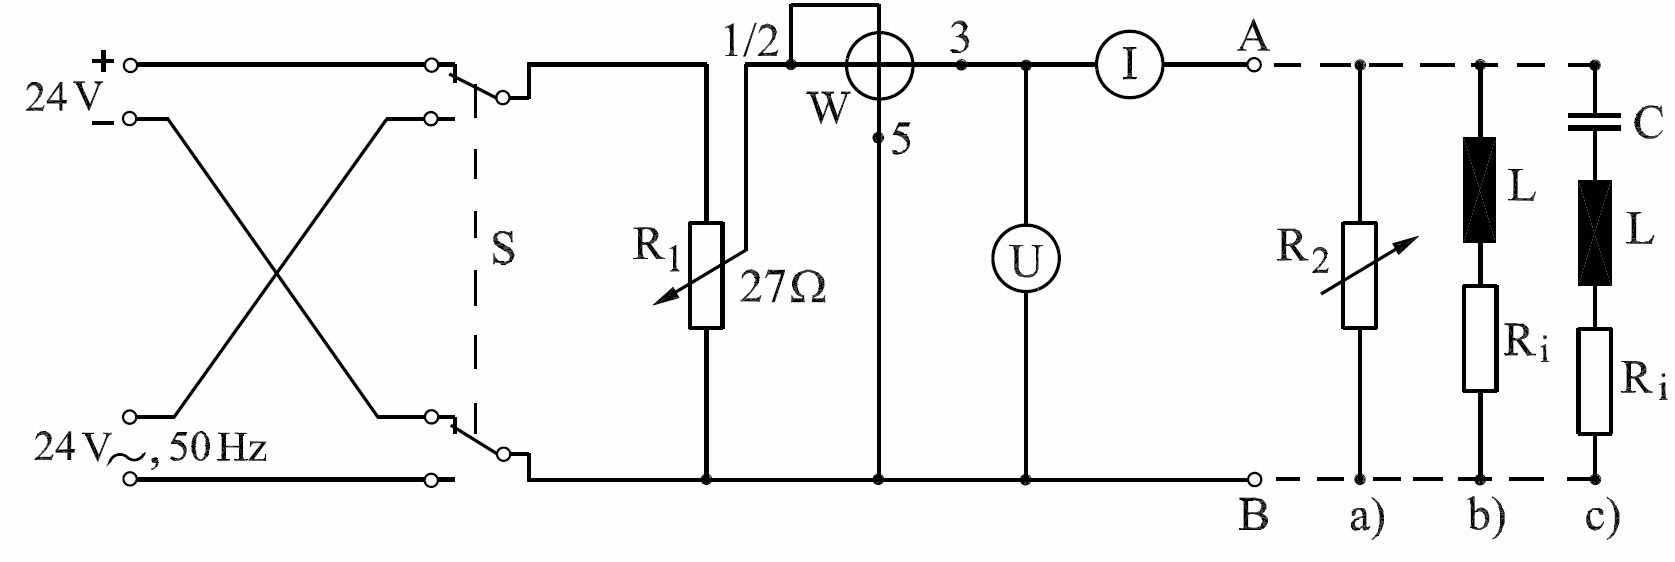
\includegraphics[width=0.9\textwidth]{auswertung/Schaltung2.png}
	\caption{Diese Schaltskizze stellt den Aufbau des Versuchs dar. Eingezeichnet sind die verschiedenen Verbraucher a), b) und c), welche in dem Versuch betrachtet werden.}
	\label{fig:Schaltskizze}	
\end{figure}
Zunächst wird die Leistung ohne angeschlossenen Verbraucher, also die Verlustleistung, für Gleich- und Wechselstrom gemessen. 
Dann werden verschiedene Verbraucher angeschlossen und für diese die Leistung, die Spannung und der elektrische Strom gemessen.
Auch dies erfolgt für Gleich- und Wechselstrom.
Bei den verwendeten Verbrauchern handelt es sich um einen Widerstand $R_2$, dann um eine Spule $L$ mit Innenwiderstand $R_i$ und zuletzt um dieselbe Spule, jedoch mit zusätzlich angeschlossenem Kondensator.
Für den letzten Fall wird nur bei Wechselstrom gemessen, da bei diesem Fall zusätzliche Effekte zum Tragen kommen.

\subsubsection{Unsicherheiten}

Die bei der Aufnahme der Messwerte zu berücksichtigenden Unsicherheiten treten hier bei den Angaben der Spannungsquelle, der Widerstände, des Kondensators, sowie bei dem Ablesen von den Messgeräten auf. 
Da es sich bei letzteren immer um Analoganzeigen gehandelt hat, wird die Unsicherheit dieser durch eine Dreiecksverteilung abhängig von der Genauigkeit der Skala bestimmt. 
Ansonsten werden die angegebenen Unsicherheiten verwendet, welche alle bei 10\% des dargestellten Werts liegen. Für die Spannungsquelle gab es keine Angabe, weswegen auch hier mit 10\% der angegebenen \SI{24}{\V} gerechnet werden.
Im Allgemeinen werden zur Berechnung der kombinierten Unsicherheiten die nach GUM vorgesehenen Formeln verwendet. 
Die Berechnung dieser für diesen Versuch erfolgt im Anhang (\ref*{sec:anhang}).

\subsubsection{Komplikationen}

Trotz Korrektheit der Schaltung, welche von der Betreuerin geprüft wurde, konnten keine Werte gemessen werden. 
Der Austausch des Gerätes zur Messung der Leistung löste dieses Problem.
Allerdings war es nicht möglich mit dem Multimeter, welches bereits bei den Akkumulatorzellen verwendet wurde, ohne angeschlossenen Verbraucher, eine Spannung und die zugehörige Verlustleistung zu messen.
Das Messgerät für die Leistung schlug in den negativen Bereich aus, was aus physikalischer Sicht unlogisch war.
Aus diesem Grund wurde statt des Multimeters ein einfaches Voltmeter angeschlossen.
Damit ließen sich Werte messen, jedoch auch eine Spannung von ca. \SI{25,5}{\V}, was mehr als der Eingangsspannung entsprechen würde. Da dieser Wert jedoch innerhalb der angenommenen 10\% Unsicherheit dür die Quelle liegt, wird er akzeptiert.

\subsection{Datenanalyse}

Alle aufgenommenen Werte sind dem Laborbuch zu entnehmen. 
Darüber hinaus sind die Daten in den folgenden Diagrammen graphisch dargestellt.
\begin{figure}[ht]
	
	\centering	
	\begin{subfigure}{0.70\textwidth}
		\centering
		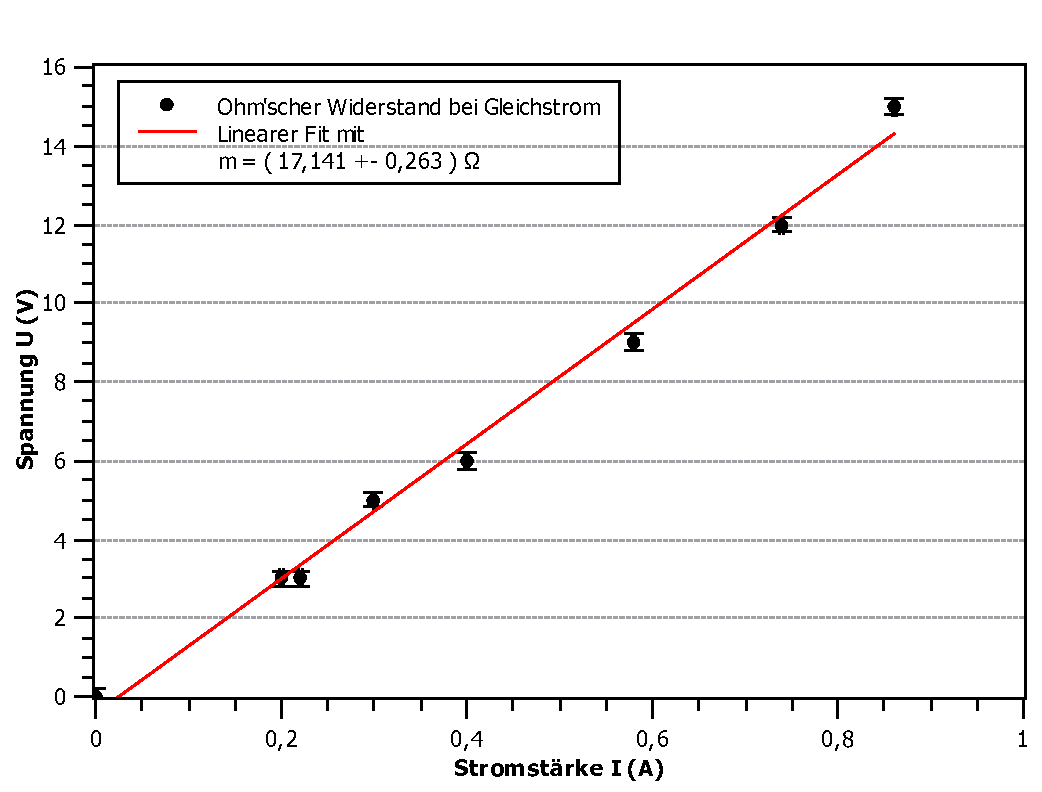
\includegraphics[width=\textwidth]{auswertung/widerstand_gleichstrom_Widerstand.pdf}
		\label{fig:1}
		\caption{Graphische Darstellungen der $U$-$I$-Kennlinie bei Gleichstrom und Widerstand als Verbraucher.}	
	\end{subfigure}
	\begin{subfigure}{0.70\textwidth}
		\centering
		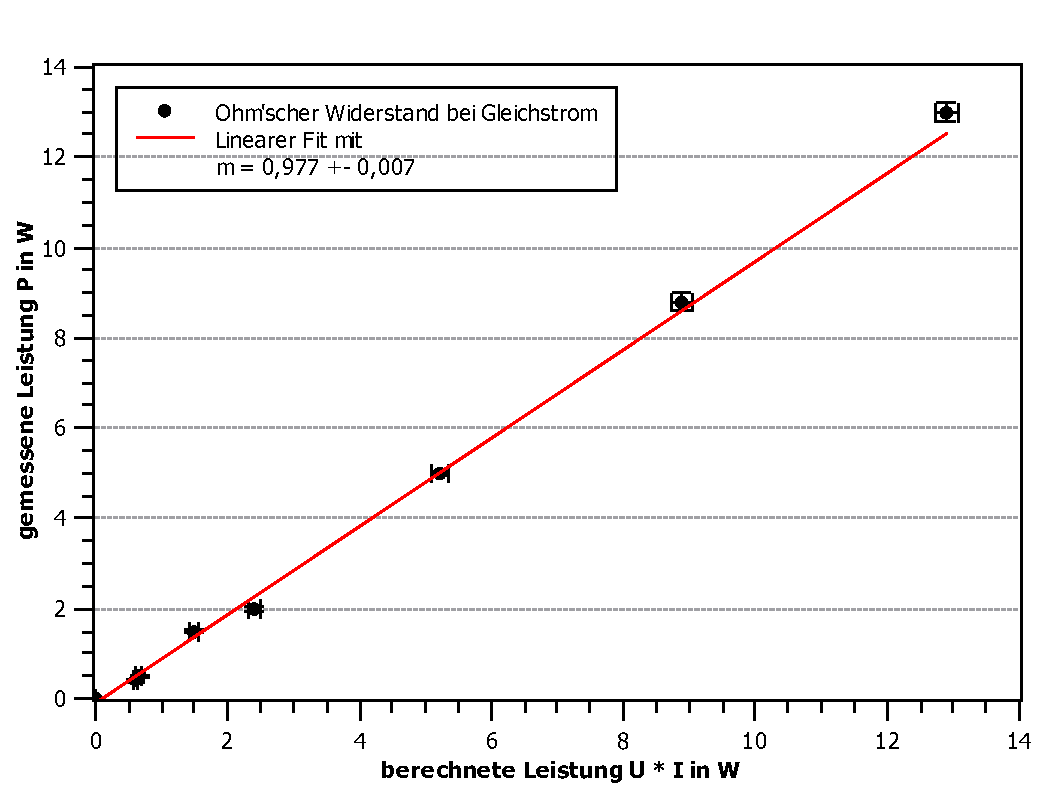
\includegraphics[width=\textwidth]{auswertung/widerstand_gleichstrom_Leistung.pdf}
		\label{fig:2}
		\caption{Verhältnis der ermittelten und gemessenen Leistung bei Gleichstrom und Widerstand als Verbraucher.}	
	\end{subfigure}
	\caption{Graphische Darstellungen der $U$-$I$-Kennlinie des Widerstands, sowie Verhältnis der ermittelten und gemessenen Leistung bei dem Widerstand als Verbraucher bei Gleichstrom.}
	\label{fig:R_gleich}
\end{figure}
\begin{figure}[ht]
	
	\centering	
	\begin{subfigure}{0.70\textwidth}
		\centering
		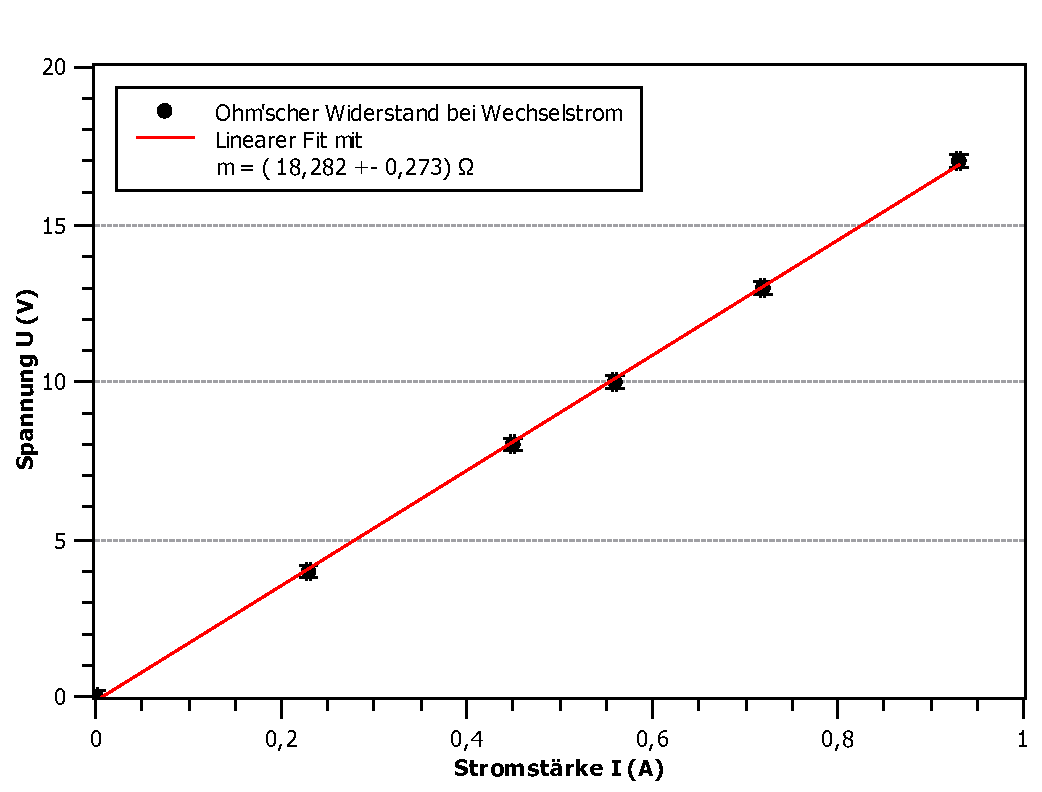
\includegraphics[width=\textwidth]{auswertung/widerstand_wechselstrom_Widerstand.pdf}
		\label{fig:3}
		\caption{Graphische Darstellungen der $U$-$I$-Kennlinie bei Wechselstrom und Widerstand als Verbraucher.}	
	\end{subfigure}
	\begin{subfigure}{0.70\textwidth}
		\centering
		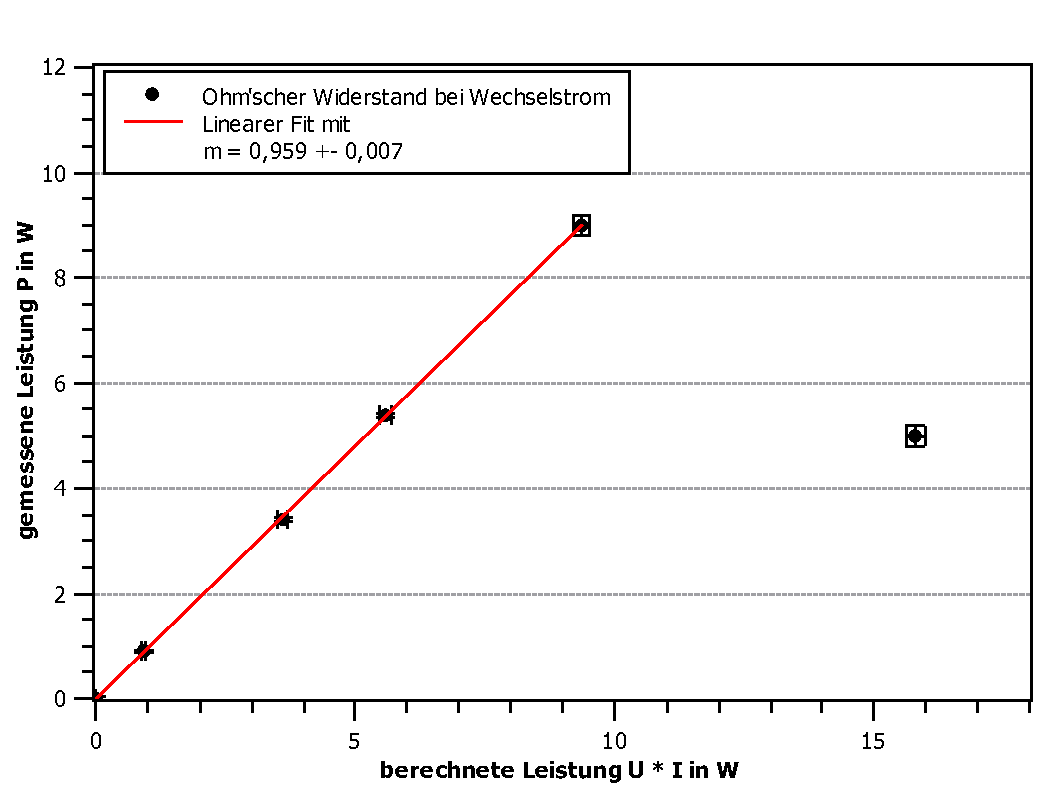
\includegraphics[width=\textwidth]{auswertung/widerstand_wechselstrom_Leistung.pdf}
		\label{fig:4}
		\caption{Verhältnis der ermittelten und gemessenen Leistung bei Wechselstrom und Widerstand als Verbraucher. Da der eine Messpunkt offensichtlich falsch aufgenommen wurde, wurde dieser nicht mit ausgewertet.}	
	\end{subfigure}
	\caption{Graphische Darstellungen der $U$-$I$-Kennlinie des Widerstands, sowie Verhältnis der ermittelten und gemessenen Leistung bei dem Widerstand als Verbraucher bei Wechselstrom.}
	\label{fig:R_wechsel}
\end{figure}
\begin{figure}[ht]
	
	\centering	
	\begin{subfigure}{0.70\textwidth}
		\centering
		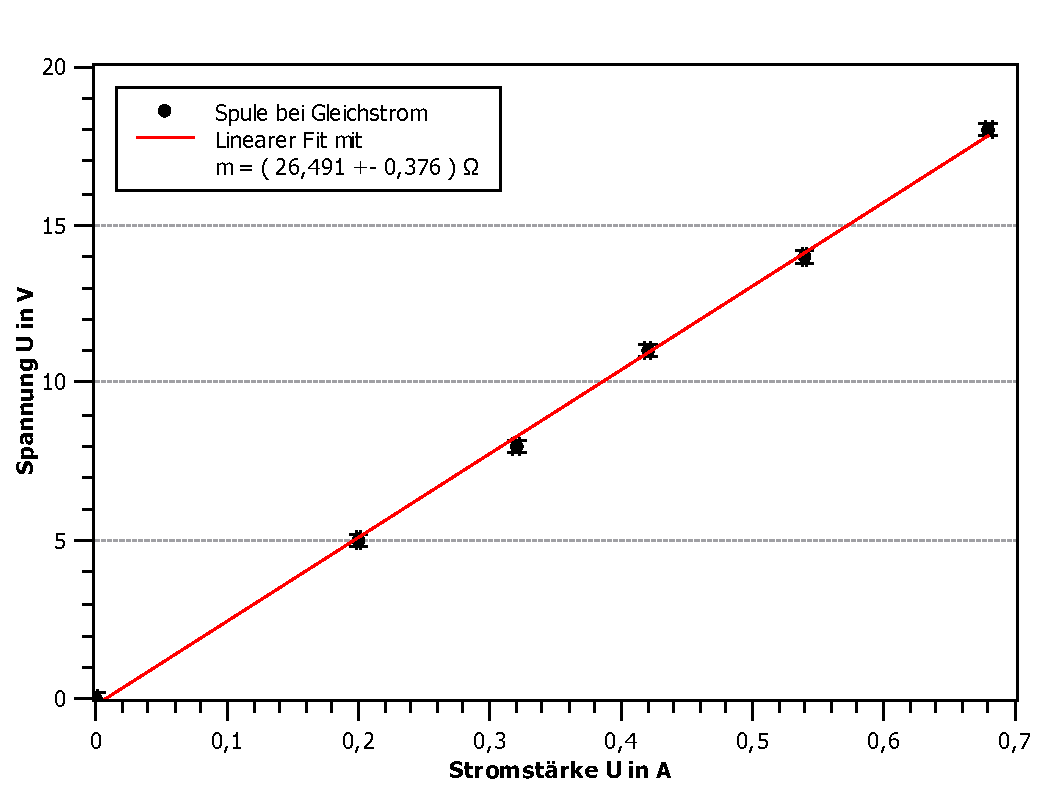
\includegraphics[width=\textwidth]{auswertung/spule-gleich-Widerstand.pdf}
		\label{fig:5}
		\caption{Graphische Darstellungen der $U$-$I$-Kennlinie bei Gleichstrom und Spule als Verbraucher.}	
	\end{subfigure}
	\begin{subfigure}{0.70\textwidth}
		\centering
		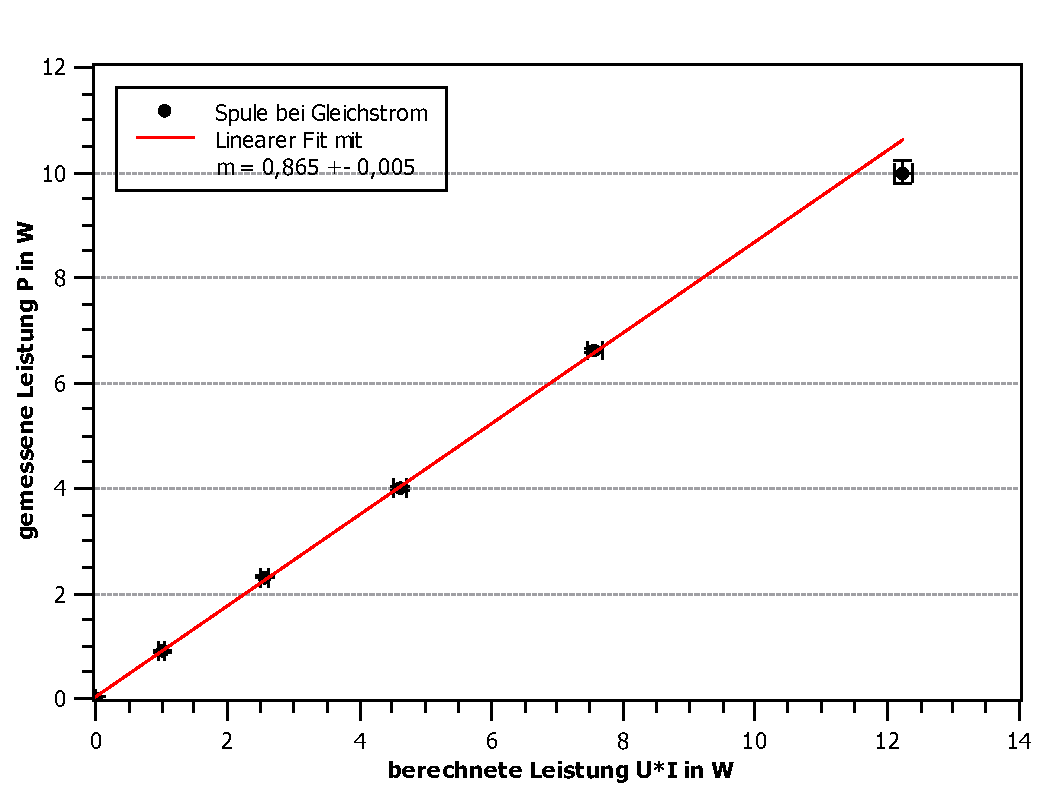
\includegraphics[width=\textwidth]{auswertung/spule-gleich-Leistung.pdf}
		\label{fig:6}
		\caption{Verhältnis der ermittelten und gemessenen Leistung bei Gleichstrom und Spule als Verbraucher.}	
	\end{subfigure}
	\caption{Graphische Darstellungen der $U$-$I$-Kennlinie des Widerstands, sowie Verhältnis der ermittelten und gemessenen Leistung bei der Spule als Verbraucher bei Gleichstrom.}
	\label{fig:Spule_gleich}
\end{figure}
\begin{figure}[ht]
	
	\centering	
	\begin{subfigure}{0.70\textwidth}
		\centering
		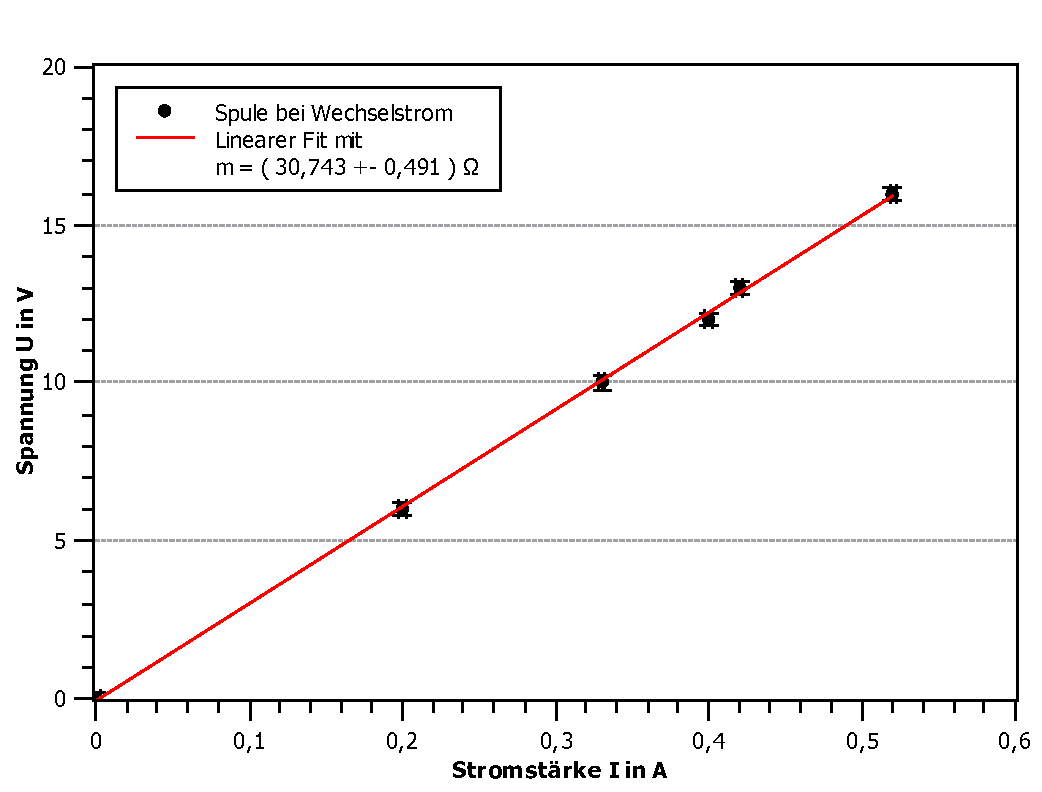
\includegraphics[width=\textwidth]{auswertung/spule-wechsel-Widerstand.pdf}
		\label{fig:7}
		\caption{Graphische Darstellungen der $U$-$I$-Kennlinie bei Wechselstrom und Spule als Verbraucher.}	
	\end{subfigure}
	\begin{subfigure}{0.70\textwidth}
		\centering
		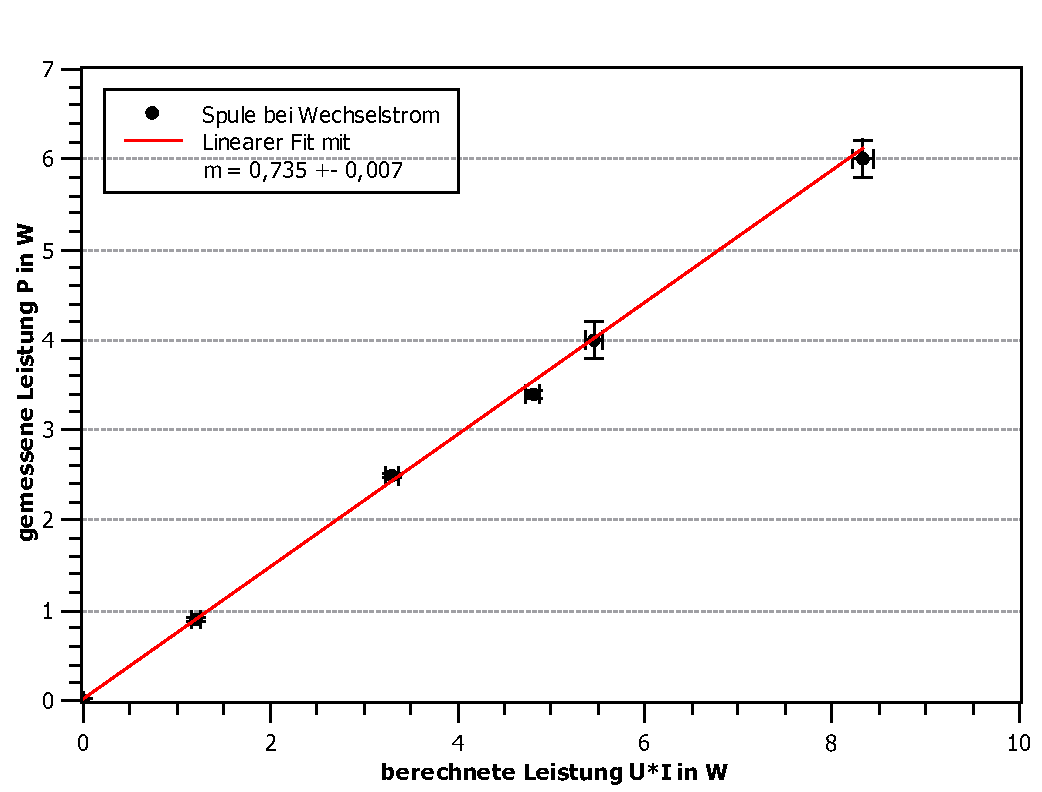
\includegraphics[width=\textwidth]{auswertung/spule-wechsel-Leistung.pdf}
		\label{fig:8}
		\caption{Verhältnis der ermittelten und gemessenen Leistung bei Wechselstrom und Spule als Verbraucher.}	
	\end{subfigure}
	\caption{Graphische Darstellungen der $U$-$I$-Kennlinie des Widerstands, sowie Verhältnis der ermittelten und gemessenen Leistung bei der Spule als Verbraucher bei Wechselstrom.}
	\label{fig:Spule_wechsel}
\end{figure}
\begin{figure}[ht]
	
	\centering	
	\begin{subfigure}{0.70\textwidth}
		\centering
		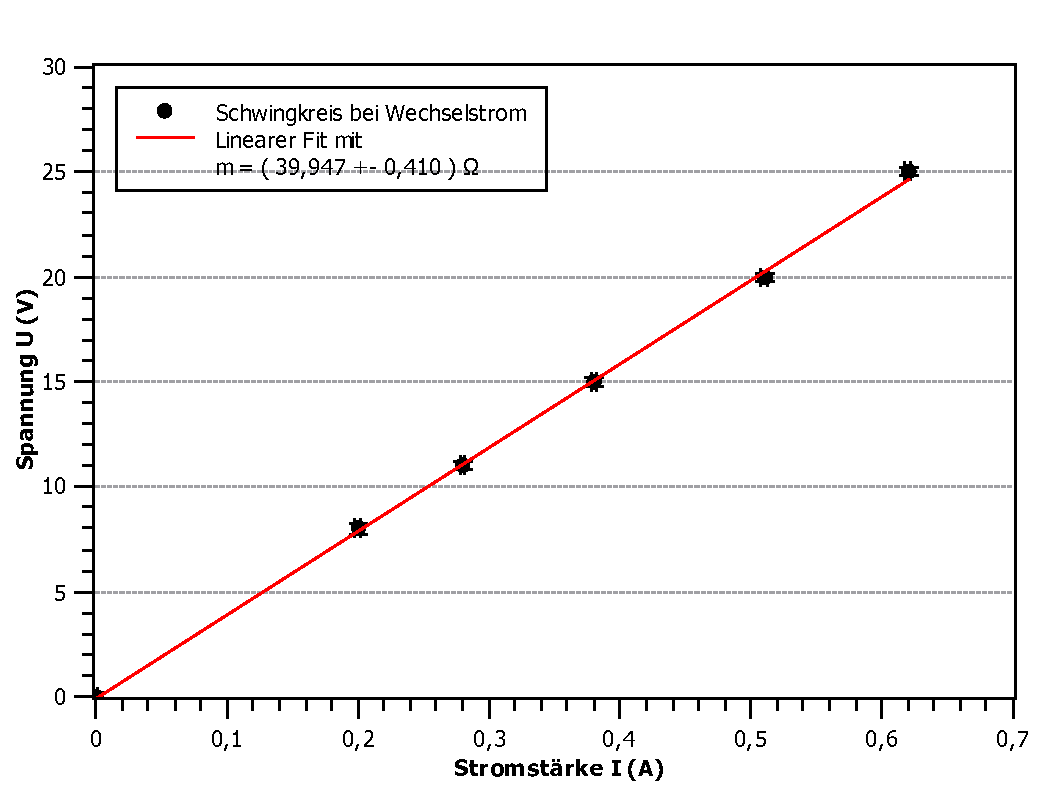
\includegraphics[width=\textwidth]{auswertung/kondensator-wechsel-Widerstand.pdf}
		\label{fig:9}
		\caption{Graphische Darstellungen der $U$-$I$-Kennlinie bei Wechselstrom und Kondensator und Spule als Verbraucher.}	
	\end{subfigure}
	\begin{subfigure}{0.70\textwidth}
		\centering
		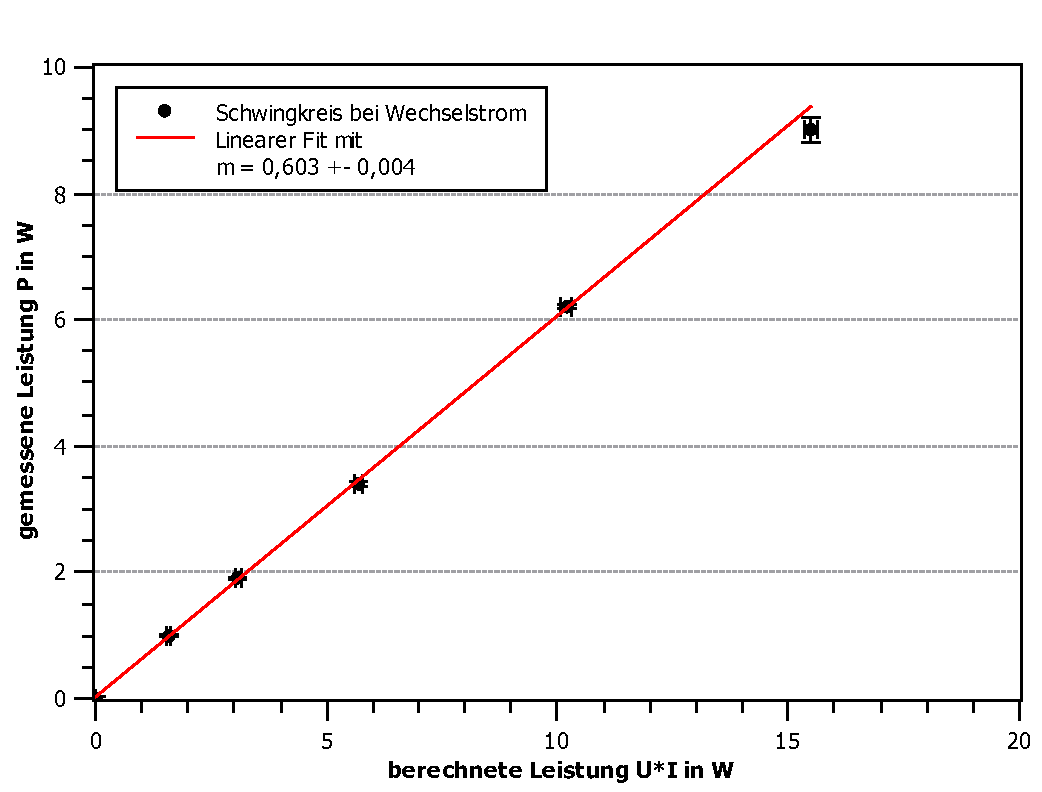
\includegraphics[width=\textwidth]{auswertung/kondensator-wechsel-Leistung.pdf}
		\label{fig:10}
		\caption{Verhältnis der ermittelten und gemessenen Leistung bei Wechselstrom und Kondensator und Spule als Verbraucher.}	
	\end{subfigure}
	\caption{Graphische Darstellungen der $U$-$I$-Kennlinie des Widerstands, sowie Verhältnis der ermittelten und gemessenen Leistung bei dem Kondensator und der Spule als Verbraucher bei Wechselstrom.}
	\label{fig:schwing_wechsel}
\end{figure}
Zunächst wurde die Verlustleistung bestimmt, dazu wurde der Schaltkreis ohne Verbraucher verwendet. 
Das Messgerät für die Leistung zeigte \SI{1,1+-0,2}{\W} bei \SI{23,5+-0,2}{\V} und Wechselstrom. 
Bei Gleichstrom waren dies \SI{2,2+-0,2}{\W} bei \SI{25,5+-0,2}{\V}.
Für die drei Verbraucher wurden in den Abbildungen \ref{fig:R_gleich} bis \ref{fig:schwing_wechsel} immer die $U$-$I$-Kennlinien und die Verhältnisse zwischen der gemessenen Leistung und der aus $P = UI$ berechneten graphisch dargestellt.
Aus den $U$-$I$-Kennlinien lassen sich die Widerstände der Verbraucher ermitteln. Diese entsprechen der Steigung der berechneten linearen Fits. Für die Spule handelt es sich hierbei bei Wechselstrom um den Scheinwiderstand $|Z|$ und bei Gleichstrom um den ohm'schen Widerstand $R_i$.
Da bei Wechselströmen die gemittelte Leistung über die effektiven Spannungen und Stromstärken gemäß der folgenden Formel definiert ist:
\begin{align}
	\bar{P} = U_{eff}I_{eff}\cos{\varphi} \\
	\varphi = \arccos{\left( \frac{\bar{P}}{U_{eff}I_{eff}}\right) },
\end{align}
lässt sich der Phasenwinkel $\varphi$ aus dem Verhältnis der gemessenen Leistung und dem Produkt der gemessenen Spannung und Stromstärke bestimmen. Der Wirkwiderstand ist gleich dem Scheinwiderstand multipliziert mit dem Kosinus der Phase $R_W = |Z|\cos(\varphi)$.
Mit der Frequenz der Spannugsquelle von \SI{50}{\Hz} ergibt sich eine Kreisfrequenz $\omega$ von \SI{314,16}{\s^{-1}}.
Die Induktivität $L$ der Spule ergibt sich aus dem folgenden Zusammenhang:
\begin{align}
	L = \frac{|Z|}{\omega sin(\varphi)}. 
\end{align}
Und zuletzt die Kapazität des Kondensators:
\begin{align}
	C = \frac{1}{\omega}\frac{1}{(\omega L - |Z|\sin (\varphi))}. 
\end{align} 
Für die Phase des Kondensators wird die gleiche Formel wie oben verwendet, jedoch mit negativem Vorzeichen, da die Phasenverschiebung der Spule umgekehrt ist.
In der folgenden Tabelle sind alle relevanten Ergebnisse der Messungen aufgezeichnet:
\begin{table}[ht]
	\caption{In dieser Tabelle sind die gemessenen und ermittelten Werte verzeichnet.}
	\centering
	\label{tab:Messwerte}
	
		\begin{tabular}{l l}
			\begin{tabular}{l|c}
				{Größe} & {Wert}	\\
				\hline
				{Verbraucherwiderstand bei Gleichstrom $R_{2,gl}$} & {\SI{17,141+-0,263}{\ohm}} \\
				{Verbraucherwiderstand bei Wechselstrom $R_{2,w}$} & {\SI{18,282+-0,273}{\ohm}} \\
				{Wirkwiderstand $R_w$ Spule} & {\SI{22,589+-0,419}{\ohm}} \\
				{Ohm'scher Widerstand $R_i$ Spule} & {\SI{26,491+-0,376}{\ohm}} \\
				{Phasenwinkel $\varphi$ Spule} & {\SI{0,745+-0,010}{}} \\
				{Induktivität $L$ Spule} & {\SI{0,066+-0,001}{\henry}} \\
				{Kapazität $C$ Kondensator} & {\SI{0,060+-0,001}{\milli\farad}} \\
				{Scheinwiderstand $|Z|$ Kondensator + Spule} & {\SI{39,947+-0,410}{\ohm}} \\
				{Phasenwinkel $\varphi$ Kondensator + Spule} & {\SI{-0,923+-0,005}{}} \\
			\end{tabular}	
		\end{tabular}

\end{table}

\subsection{Diskussion}

Die Betrachtung des Widerstands bei Gleich- und Wechselstrom zeigt, dass der Widerstand bei letzterem größer ist, dies liegt daran, dass bei Wechselstrom der Scheinwiderstand gemessen wird und zusätzlich noch der Imaginärteil zum Tragen kommt.
Dasselbe gilt für die Spule. 
Vergleicht man bei dieser jedoch den Wirkwiderstand mit dem ohm'schen, so fällt auf, dass dieser kleiner ist.
Der Wirkwiderstand ist dabei der Realanteil des Scheinwiderstandes und abhängig von der Phase ändert sich dieses Verhältnis.
Da der Kondensator aus drei parallel geschalteten Kondensatoren mit jeweils \SI{0,020+-0,002}{\milli\farad} bestand, addieren sich diese der Theorie nach für die Gesamtkapazität zusammen (\SI{0,060+-0,004}{\milli\farad}). 
Dieser Wert stimmt eindeutig mit dem ermittelten überein.

Demnach gibt es eine Übereinstimmung mit der Theorie. 
Es sind also keine nennenswerte Abweichungen gemessen worden. 

\subsection{Schlussfolgerung}

Die Messergebnisse deuten auf eine Bestätigung der Theorie hin. 
Alle gemessenen Werte stimmen nämlich mit den Erwartungen überein. 
Das Ziel dieses Versuches wurde demnach erreicht und eine Wiederholung ist somit nicht notwendig.
Die Betrachtung der Unsicherheiten schließt ebenfalls starke Abweichungen aus, da diese sehr genau sind.
